% THIS IS SIGPROC-SP.TEX - VERSION 3.1
% WORKS WITH V3.2SP OF ACM_PROC_ARTICLE-SP.CLS
%
% REMEMBER HOWEVER: After having produced the .bbl file,
% and prior to final submission,
% you need to 'insert'  your .bbl file into your source .tex file so as to provide
% ONE 'self-contained' source file.
\documentclass{acm_proc_article-sp}
\usepackage{url}
%\usepackage{listings}

\begin{document}

\title{Growing up with Nell: A Narrative Interface for Literacy}
%\subtitle{Narrative Interfaces for Literacy}
%
% You need the command \numberofauthors to handle the 'placement
% and alignment' of the authors beneath the title.
%
% For aesthetic reasons, we recommend 'three authors at a time'
% i.e. three 'name/affiliation blocks' be placed beneath the title.
%
% NOTE: You are NOT restricted in how many 'rows' of
% "name/affiliations" may appear. We just ask that you restrict
% the number of 'columns' to three.
%
% Because of the available 'opening page real-estate'
% we ask you to refrain from putting more than six authors
% (two rows with three columns) beneath the article title.
% More than six makes the first-page appear very cluttered indeed.
%
% Use the \alignauthor commands to handle the names
% and affiliations for an 'aesthetic maximum' of six authors.
% Add names, affiliations, addresses for
% the seventh etc. author(s) as the argument for the
% \additionalauthors command.
% These 'additional authors' will be output/set for you
% without further effort on your part as the last section in
% the body of your article BEFORE References or any Appendices.

\numberofauthors{1}
\author{
% You can go ahead and credit any number of authors here,
% e.g. one 'row of three' or two rows (consisting of one row of three
% and a second row of one, two or three).
%
% The command \alignauthor (no curly braces needed) should
% precede each author name, affiliation/snail-mail address and
% e-mail address. Additionally, tag each line of
% affiliation/address with \affaddr, and tag the
% e-mail address with \email.
%
% 1st. author
\alignauthor
C. Scott Ananian\\
\affaddr{One Laptop Per Child Foundation}\\
\affaddr{222 Third Street}\\
\affaddr{Cambridge, MA 02142}\\
\email{cscott@laptop.org}
%\and  % use '\and' if you need 'another row' of author names
}
\date{12 March 2012}
% Just remember to make sure that the TOTAL number of authors
% is the number that will appear on the first page PLUS the
% number that will appear in the \additionalauthors section.

\maketitle

\begin{abstract}
Project Nell is tablet software to teach reading and writing to
children far from educational infrastructure.  Nell is a modular
narrative system with ``a low floor and no ceilings'': the design
scales from teaching letter shapes to programming the system itself.

Nell is the successor to the Sugar educational software developed by
One Laptop per Child for their XO-1 laptop.  Nell targets the XO-3
tablet, a sub-\$100 solar-powered tablet for the developing world.
%Experience with Sugar drove design choices for Nell.

\textbf{XXX REWRITE THE ABSTRACT XXX}
\end{abstract}

% A category with the (minimum) three required fields
\category{K.3.1}{Computers and Education}{Computer
  Uses in Education}[computer-managed instruction]
\category{I.2.7}{Artificial Intelligence}{Natural Language
  Processing}[narrative interfaces]
\category{H.5.2}{Information Interfaces and Presentation}{User
  Interfaces}[narrative interfaces]
\terms{Design, Human Factors}

\keywords{Narrative interfaces, tablet computing, education, Nell}

\section{A Lesson from Nell}
\begin{figure}
\centering
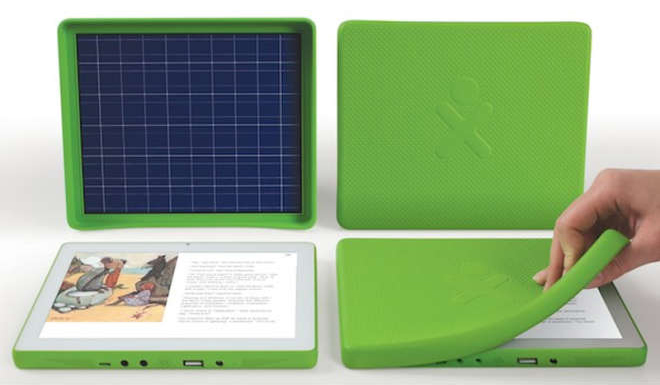
\epsfig{file=xo3-3.eps, width=3.2in}
\caption{Nell's solar-powered hardware platform.  The tablet design
  allows for direct interaction.}\label{fig:xo3}
\end{figure}
% tell a nell story up front
Miles from the nearest school, a young Ethiopian girl turns on a
tablet computer for the first time.  The solar-powered machine begins
talking to her immediately: \textit{``Hello!  Would you like to hear a story?''}

She nods and listens to a story about a princess.  Later, when
the girl has learned a little more, she will tell the machine that the
princess is named ``Rahel,'' like she is, and change all its
colors---but for now the green book draws pictures of the unnamed Princess
for her and asks her to trace shapes on the screen.

\textit{``R is for Raven.  Can you trace the R?''}

As she traces the R, it comes to life and gallops across the screen.
\textit{``Run starts with R.  Roger the R runs across the Red Rug.  Roger has a
dog named Rover.''}  Rover barks: \textit{``Ruff! Ruff!''}  The Princess asks,
\textit{``Can you find something Red?''} and Rahel uses the camera to
photograph her new boots.

\textit{``Very good!  You are a smart girl!''}

As Rahel grows, the book asks her to trace not just letters, but whole
words.  The book's responses are written on the screen as it speaks
them, and eventually she doesn't need to leave the sound on all the
time.  Soon Rahel can write complete sentences in her special book,
and sometimes the Princess will respond to them.  New stories teach her about
music (she unlocks a dungeon door by playing certain tunes) and
programming with blocks (Princess Rahel helps a not-very-bright turtle
to draw different shapes).  Rahel writes her own stories about the Princess,
which she shares with her friends.

An older Rahel learns that the block language she used to talk with
the turtle is also used to write all the software running inside
her special book.  The stories Rahel writes can now include new
functionality that make her book even more exciting for the kids
just now receiving their own green meta books.

\section{Key Ideas}
The interaction design of the Nell system described above is inspired
by the ``Young Lady's Illustrated Primer'' in the Neal Stephenson
novel \textit{The Diamond Age}, from whose protagonist Nell takes its
name.\footnote{In a nod to Seymour Papert, Nell can also be read as an
acronym for ``Narrative Environment for Learning Learning.''}
Nell's design embodies four key ideas: it is a \textbf{Narrative}
interface using \textbf{Direct Interaction} which \textbf{Grows} with,
and is \textbf{Personalized} for, the child.

We believe the combination of these four key concepts provides a novel
experience which addresses some of the shortcomings of earlier
learning environments for children.  In this section we will discuss
these four building blocks, and in the next section we will describe their
implementation in Nell.

%Section~\ref{sec:related} discusses related work.
%The final section will draw conclusions and describe future work.

\subsection{Narrative}

Experience with our previous educational software
system~\cite{flores:uruguay,idb:peru} has shown gratifying uptake and
use by children.  But we are often disappointed that some of our
favorite pedagogical tools included in the systems were not being
widely used.  Enthusiastic teachers would spark intensive use in
certain classrooms, but children had difficulty finding their way into
the material without strong guidance.

Children (like all humans) are hard-wired for
stories~\cite{boyd:stories}.  Nell uses a
\textit{Narrative Interface}~\cite{bizzocchi:narrative,don:narrative,laurel:computers} 
to guide the child user through the pedagogical capabilities of the
system.  All system actions are shaped by the storybook metaphor, and
interactions with the system are conceptualized as interactions with
one of the system protagonists.

Nell's overall story is a multi-character serial adventure, taking
cues from \textit{The Diamond Age} and
from the UNIVERSE narrative-generation system \cite{lebowitz:universe84}.
Each of the several characters represents a specific skill or subject
area, and each adventure represents about a year's curriculum.  This
design also improves modularity and allows updates and decentralized
authorship.

\begin{figure}
\centering

\epsfig{file=roger1.eps, height=1.5in} % width=3.2in
\caption{Illustration of Nell's primary interface.}\label{fig:nell}
\end{figure}

As illustrated in figure~\ref{fig:nell}, Nell's characters are
always-available agents layered above a particular system \textit{activity}
(application) which provides specialized functionality.  The agents
are not always foregrounded: constructionist learning occurs when the
child plays freely to ``make things'' with the base activity.
The handwriting tutor is fundamentally a drawing activity; the
adventure involving the magical musical lock is also a music-making activity.
%  ``Making things'' is the key to constructionist learning.
The narrative system is
hooked into each activity to provide passive guidance
(congratulating the child when it notices they've drawn a letter),
active guidance (Apple-Guide--style~\cite{powers:appleguide}
contextual help), or system services (switch activities; jump into a
related story module/lesson plan).

% Story Module == Lesson Plan

% not always a story -- kid can draw on their own and return to the
% story; Nell will observe the free play and offer suggestions.
\subsection{Personalized}
% customization, renaming characters

Children often decorate their belongings, and the
child owning a Nell system is encouraged to personalize it.
Superficially, colors can be changed and characters can be renamed and
dressed up.  But Nell also supports deeper story personalization.

\textit{Avatar Services} stores all choices made by the child and make them
accessible to story modules and activities.  Accomplishments
(completed lessons) are also stored.  Nell can thus provide multiple
alternative story modules for a given plot point/lesson, and select
between them based on either the explicit choices made by the child
(``fractions in outer space,'' if the child previously indicated a
preference for space-themed lessons) or prior success with a given
lesson style (a large number of accomplishments in musical-rhythmic
tasks suggests a rhythmic approach to fractions).  In this manner we
can engage the child's interests and cater to different learning
styles~\cite{gardner:mi}.

Moving further, this record of past choices and accomplishments can be
reviewed.  The narrative history is stored in the \textit{Journal},
where it can form the core of a Portfolio~\cite{stefanakis:portfolios}.
In order to encourage fearless play and experimentation, the Journal
also supports pervasive undo; you can replay the narrative starting at
any past point in the journal.

In the future, we expect to allow further narrative personalization
via recombination of story elements.
Lebowitz~\cite{lebowitz:universe85} and Riedl~\cite{riedl:planning}
show how a planner can be used to recombine and adapt story fragments.
In this we expect to be less ambitious than the cited work: instead of
attempting to generate thousands of stories from tens of templates, we
expect to select and then modestly adapt from hundreds of story
modules created in a decentralized manner by teachers---and eventually
by the students themselves.

\subsection{Growable}
The Nell system aims to have a ``low floor and no ceiling.''  The low
floor is a very simple base system, usable with no literacy skills or
external guidance.  The system then grows with the child's expanding
capabilities, serially accumulating story modules to tackle topics of
increasing difficulty.  As mentioned before, the ability for third
parties to independently author story modules is necessary to ensure
Nell can continue to grow.  There should be no external dependencies
limiting a child's ability to participate in this process: a Nell
system contains a story editor and everything necessary to
author and publish story modules.

We also seek to eliminate the ``ceiling'' between the children and
the authors of the Nell system itself.  Nell should be capable of
teaching about itself, and a capable child can dive into Nell's source
code and make meaningful changes.  In section~\ref{sec:turtles} we
describe how this goal is approached.

% it has a ``low floor and no ceiling'' to allow a child to master more
% and more of the system as she grows.
% modular -- the story expands.
% text read aloud initially

\subsection{Direct interaction}
% constructionist?
% handwriting as UI?
% motor skills
% photo of XO-3?

The constructionist learning philosophy emphasizes creation and
tangible interaction.  Nell uses direct interaction on a tablet
computer to maintain the child's connection to their work
(Figure~\ref{fig:xo3}).

The direct interaction model lowers the floor by eliminating the need
to learn an abstract touchpad or mouse interface.  It also supports
our literacy goals by allowing direct handwriting instruction and the
use of handwriting as an interface.

\section{Technology}
We have begun implementation of the Nell system.  In this section we
will describe the implementation of three of the most novel pieces
from the software engineering side.  These are not necessarily the
most novel-appearing from the user's perspective: for example, the
handwriting UI is still fairly unusual in consumer devices, but the
implementation of a separated-character handwriting recognition engine
using Hidden Markov Models is well-understood.
\textbf{SMOOTH THIS LANGUAGE}

\subsection{Rule-based story modules}
\begin{figure}\small
\begin{verbatim}
{ world: { // id gives canonical URL for this module
    id: "/nell.laptop.org/chapters/alphabet-book"
    scene: "opening", // initial scene
  }, scenes: [
    { id: "opening", subject: "actors/princess",
      verb: "speak", object: "actors/user",
      text: "Hello! Would (o/2) like to hear a story?"
    },
    { id: "story-1",
      cond: rule`At(opening) && Event(Chat, Yes)`,
      subject: "actors/princess",
      verb: "speak", object: "actors/user",
      text: "Once upon a time..." },
    ...
    { id: "r-drawn",
      cond: rule`Event(Activity, DrawR)`,
      subject: "actors/princess",
      verb: "speak", object: "actors/user",
      text: "Very good, (o/3)!",
      action: js`startAnimation("r-runs")` },
    ...
  ], ... }
\end{verbatim}
\caption{Excerpt of story module.  JSON syntax has been extended with
quasiquote~\cite{quasiquote}.}\label{fig:rules}
\end{figure}
Narrative is the core of the Nell interface.  It is important that
Nell's story be modular and extensible.  We use a rule-based story
model with programmable conflict resolution to provide this ability.
Figure~\ref{fig:rules} shows an excerpt of the story module driving
the interaction described in the introduction to this paper.

XXX stories consist of elements.  all elements contain preconditions,
and actions.  cite PLANNER.

In principle, all rules for all elements of all stories are evaluated
continuously to determine the actions of the narrative agents.  This
is made computationally efficient using the Rete
algorithm~\cite{rete}.  The Rete algorithm requires that our
conditions are in Normal Form\footnote{BE PRECISE HERE}, but actions
can be arbitrarily complex.

New story modules can be incorporated by visiting an internet page in
connected deployments.  In a disconnected deployments, new stories
might be distributed once a year on USB sticks, or shared from your
friends.  In a classroom environment, a teacher can share stories for
the day's lesson at the start of class.

Story modules can be inherited and extended, as figure~\ref{fig:rules2}
shows.  This makes it easy to take an existing story and modify it to
better suit particular interests or a particular type of learner, or
just to add variety.  This can lead to conflicts: multiple versions of
a story, or multiple variant elements within a story, may have their
preconditions satisfied simultaneously.

We resolve conflicts...

We have not yet implemented an integrated story editor within Nell,
but we expect it to be roughly similar to the one implemented for
Wide Ruled, which showed good learnability by inexperienced
users~\cite{wideruled}.

% excerpt of story model
% rete algorithm, cite Riedl, etc.
% programmable conflict resolution
% cite the story editor from Wide Ruled

\subsection{Extensible dialog}
The child can interact with the Princess, and other agents within
Nell, directly.  Convincing discourse is a hard problem, but
reasonable approximations do not have to be difficult; even
the rudimentary conversational abilities of ELIZA elicited hours of
conversation~\cite{weizenbaum:power}.
% her secretary is divulging her life story
% asks him to leave the room so he could be alone with it
% hours discussing her boyfriend.
Nell's use as an interactive diary is enhanced by the child's
collaboration in the fiction that Nell is intelligent---what
Turkle~\cite{turkle:alone} calls the ``ELIZA effect.''

We leverage AIML~\cite{aiml:2005},%
\footnote{Wilcox identifies several shortcomings with the expressive
  power of AIML, proposing ChatScript as a
  replacement~\cite{wilcox:2010}.  At present AIML's community and
  diversity of third-party implementations make it preferable.}
the markup language developed for AliceBot, three-time winner of the
Loebner Prize, a restricted Turing Test competition for chat bots.

\begin{figure}\small
\begin{verbatim}
<aiml version="1.0">
<category>
 <pattern>GO *</pattern>
 <template><srai><star/></srai></template>
</category>

<category>
 <pattern>N</pattern>
 <template><srai>NORTH</srai></template>
</category>

<category>
 <pattern>NORTH</pattern>
 <template>
  <javascript>FireEvent(Chat, "North")</javascript>
 </template>
</category>
</aiml>
\end{verbatim}
\caption{An AIML fragment which recognizes the commands ``N'',
  ``North'', and ``Go North''.}\label{fig:aiml}
\end{figure}
% show fragment
Each story module can include AIML fragments extending the
conversational capabilities of Nell's agents.  Figure~\ref{fig:aiml}
illustrates how this can be used to implement a traditional
text adventure interaction for a particular story module.
The child can write instructions such as, ``go north,'' ``go
east,'' or ``open door'' for the agent.  These trigger events
handled by the story module to move the agent through the
adventure---for example, by causing the activity to draw a
new location, causing the agent to describe it, and shifting the
AIML topic to enable vocabulary suitable for the new location.

% xx can the activity influence which commands are active?
% yes, by shifting the topic.  AIML should have a more flexible
% topic system.

\subsection{TurtleScript}\label{sec:turtles}
Nell's implementation leverages Web technologies, including HTML5,
WebGL, and JavaScript, with extensive use of offline caching.
Resources are named by URL, even when disconnected from the
internet.  This allows third parties to manage their own namespaces
when extending Nell, and simplifies updates to story modules and
the Nell system itself.
% if the kid's going to learn some software stack, this seem like a
% fine one to learn

As far as possible, Nell is implemented in JavaScript.  We have
developed a block-oriented view of JavaScript, which we call
TurtleScript~\cite{turtlescript}.  Combined with subsets of JavaScript
for beginners, this allows us to use a single implementation language
which scales from logo-like tasks all the way through the
implementation of the entire Nell system itself.  TurtleScript's block
view of JavaScript is isomorphic to the standard textual
representation of code.  We have begun implementation of a full
programming environment for TurtleScript which is naturally-suited to
tablet machines.

% XXX refer to TurtleScript excerpt in figure somewhere here.

Our goal is to allow the child to eventually dig as far into Nell's
implementation as their capabilities allow.  Although the operating system and
the browser itself are inaccessible from the web platform, we can
provide full access above that level.  The existence of meta-circular
interpreters for JavaScript~\cite{narcissus} implies that we can
expose the system all the way down to the programming language
implementation.  Via TurtleScript, this code is all visible in a
friendly block-based form.

% Javascript/HTML5
% offline caching
% turtles (almost) all the way down (turtlescript again)
% excerpt of TurtleScript

\section{Related work}\label{sec:related}

The TinkRBook system~\cite{chang:tinkrbook} shares a similar focus on
personalization and literacy.  Project Nell attempts to scale these
ideas with a modular extensible narrative system and a broader range
of pedagogic material.

The Sugar Learning environment~\cite{sugarXXX} is an earlier effort at
child education.  We've learned directly from this effort.  Nell
focuses on children even further from educational infrastructure.
The narrative at Nell's code attempts to provide students additional
pedagogical guidance, and the direct interaction model avoids keyboard
problems which have plagued Sugar's initial deployments.  Nell also
attempts to provide a greater sense of ownership through pervasive
customization.

Automatic narrative generation has seen attention in
gaming, simulation, and training contexts~\cite{riedlXXX}.  Nell's
use of these ideas in a pedagogical context is unique.

\section{Conclusions}
We have described the design of a novel narrative direct-interface
system for teaching literacy, which is personalized for and grows with
its child owner.  Personalized direct interface engages the child, and
narrative guides them through Nell's pedagogic material.  The low-cost
solar-powered hardware allows Nell to reach further into the
least-developed areas of the world, to help those far from traditional
educational infrastructure.

We are in the process of implementing the Nell system, and expect to
do initial deployments in Africa later this year.

\section{Acknowledgments}
Nell's design evolved from experience with the Sugar system,
architected by Walter Bender, and through stimulating discussions with
Chris Ball and Angela Chang.  Chris Ball and Michael Stone contributed
to an implementation of the rule-based story model.

%
% The following two commands are all you need in the
% initial runs of your .tex file to
% produce the bibliography for the citations in your paper.
\bibliographystyle{abbrv}
\bibliography{paper}  % paper.bib is the name of the Bibliography in this case
% You must have a proper ".bib" file
%  and remember to run:
% latex bibtex latex latex
% to resolve all references
%
% ACM needs 'a single self-contained file'!
%
\balancecolumns
% That's all folks!
\end{document}

%%  LocalWords:  personalization Lebowitz
